% Copyright 2004 by Till Tantau <tantau@users.sourceforge.net>.
%
% In principle, this file can be redistributed and/or modified under
% the terms of the GNU Public License, version 2.
%
% However, this file is supposed to be a template to be modified
% for your own needs. For this reason, if you use this file as a
% template and not specifically distribute it as part of a another
% package/program, I grant the extra permission to freely copy and
% modify this file as you see fit and even to delete this copyright
% notice. 

\documentclass[10pt]{beamer}
% Replace the \documentclass declaration above
% with the following two lines to typeset your 
% lecture notes as a handout:
%\documentclass{article}
%\usepackage{beamerarticle}


\usepackage[utf8]{inputenc}
\usepackage[italian,english]{babel}
\usepackage{amssymb, amsmath}
\usepackage{wrapfig}
\usepackage{bigints}
\usefonttheme[onlymath]{serif}

%\usepackage{extsizes}
% There are many different themes available for Beamer. A comprehensive
% list with examples is given here:
% http://deic.uab.es/~iblanes/beamer_gallery/index_by_theme.html
% You can uncomment the themes below if you would like to use a different
% one:
%\usetheme{AnnArbor}
%\usetheme{Antibes}
%\usetheme{Bergen}
%\usetheme{Berkeley}
%\usetheme{Berlin}
%\usetheme{Boadilla}
%\usetheme{boxes}
%\usetheme{CambridgeUS}
%\usetheme{Copenhagen}
%\usetheme{Darmstadt}
%\usetheme{default}
%\usetheme{Frankfurt}
\usetheme{Goettingen}
%\usetheme{Hannover}
%\usetheme{Ilmenau}
%\usetheme{JuanLesPins}
%\usetheme{Luebeck}
%\usetheme{Madrid}
%\usetheme{Malmoe}
%\usetheme{Marburg}
%\usetheme{Montpellier}
%\usetheme{PaloAlto}
%\usetheme{Pittsburgh}
%\usetheme{Rochester}
%\usetheme{Singapore}
%\usetheme{Szeged}
%\usetheme{Warsaw}



%%definitions
\newcommand{\ham}{\mathcal{H}}
\newcommand{\intk}{ \bigintsss \!\!\! \text{\small{$\frac{d^2 k}{(2\pi)^2}$}}~}
%\newcommand{\intk}{ \displaystyle \int \!\!\! \text{\footnotesize{$\frac{d^2 k}{(2\pi)^2}$}}~}
\newcommand{\oa}{\hat{a}}
\newcommand{\opsi}{\hat{\psi}}
\newcommand{\bvec}[1]{\boldsymbol{#1}}
\newcommand{\lp}{_{LP}}
\newcommand{\up}{_{UP}}

\title{Superfluid properties of exciton polariton condensates in planar microcavities}
\subtitle{Colloquio IV anno}
\author[Carmelo Mordini]{Carmelo Mordini\\ \vspace{.7cm}{\tiny Supervisors\\ \vspace{-.2cm}I. Carusotto ~ R. Fazio}}

\institute[SNS] 
{
  Scuola Normale Superiore\\
  %University of Somewhere
  }
\date{Maggio 2014}


% % Delete this, if you do not want the table of contents to pop up at
% % the beginning of each subsection:
% \AtBeginSubsection[]
% {
%   \begin{frame}<beamer>{Riassunto}
%     \tableofcontents[currentsection,currentsubsection]
%   \end{frame}
% }

% Let's get started
\begin{document}

\begin{frame}
  \titlepage
\end{frame}

\begin{frame}{Outline}
  \tableofcontents
  % You might wish to add the option [pausesections]
\end{frame}

% Section and subsections will appear in the presentation overview
% and table of contents.
\section{Cavità di semiconduttori}

\subsection{Dinamica dei polaritoni}

 \begin{frame}{Cavità 2D}
 \small

\begin{minipage}{\textwidth}
  \begin{columns}
  
  \begin{column}{.6\textwidth}
    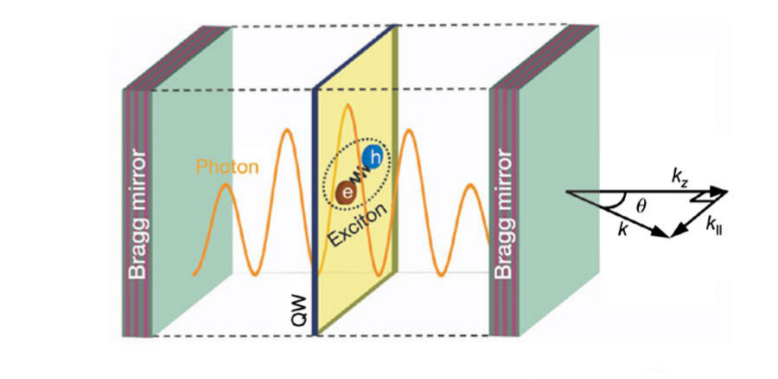
\includegraphics[scale=.2]{QW_color.png}
  \end{column}

  \begin{column}{.4\textwidth}
    Le cavità bidimensionali di semiconduttore si rivelano uno strumento potente per studiare la fisica dei fluidi quantistici.
    \end{column}
  \end{columns}
  \end{minipage}
  
  Il confinamento spaziale e l'interazione con il mezzo fanno acquistare alla luce una dinamica analoga a quella di un fluido di particelle.
  
  \begin{minipage}{\textwidth}
  \begin{columns}
  
  \begin{column}{.5\textwidth}
    \begin{itemize}
     \item Polaritoni
     \item Superfluidità
     \item Esperimenti
    \end{itemize}

  \end{column}

  \begin{column}{.5\textwidth}
  \begin{figure}
    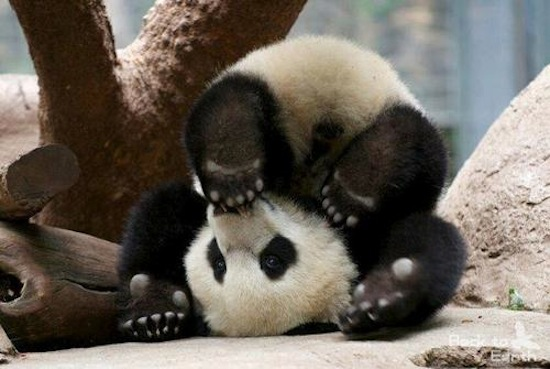
\includegraphics[scale=.2]{Panda.jpg}
  \end{figure}
    \end{column}
  \end{columns}
  \end{minipage}
  
  
 \end{frame}


\begin{frame}{Cavità 2D}%{Optional Subtitle}

    \begin{figure}
     \fbox{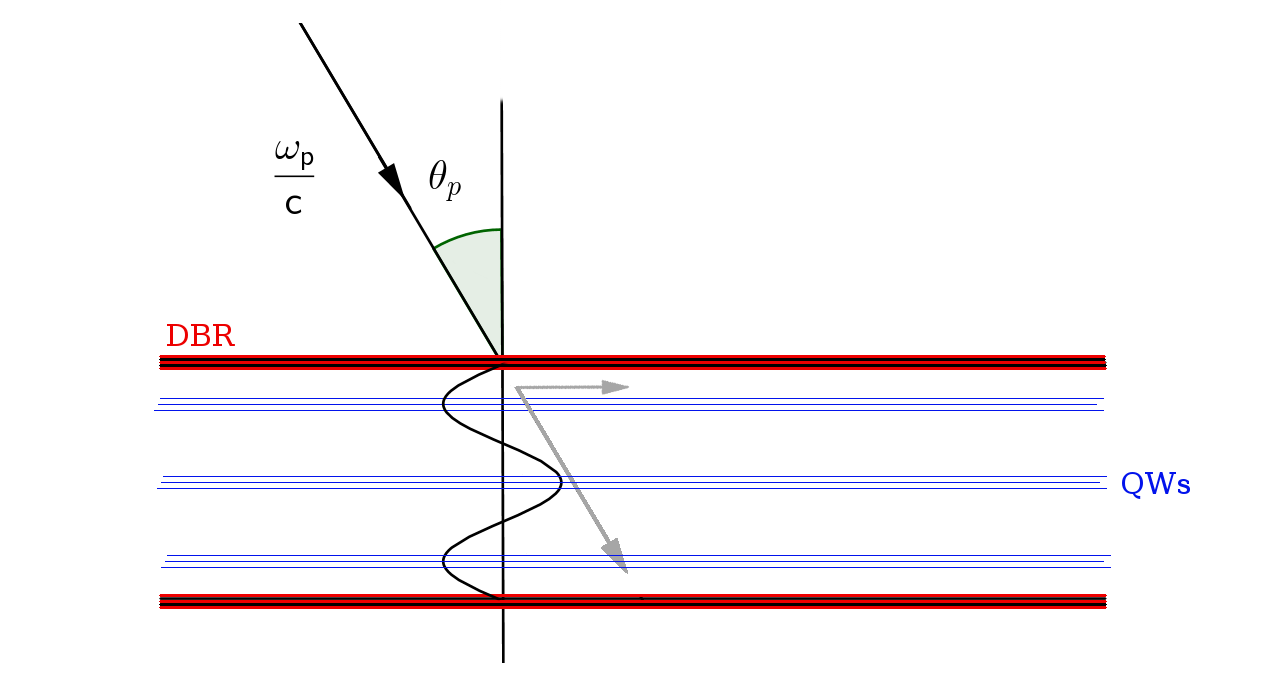
\includegraphics[scale=.7]{QW_field.png}}
    \end{figure}
    
    \begin{itemize}
     \item Massa del fotone dipendente dallo stato trasverso eccitato
    \end{itemize}
\vspace{-.5cm}        
      \begin{minipage}{\textwidth}
      \begin{columns}
	  \begin{column}{.5\textwidth}

	   \begin{align*}
	\omega_C(k) &= \frac{c}{n_0}\sqrt{{q_z}^2 + k^2} \\ 
		&\simeq \omega_C^0 + \frac{\hbar k^2}{2m_C}
	\end{align*}
	  \end{column}
	    
	  \begin{column}{.5\textwidth}
	  \footnotesize
	    $$\begin{cases}
	      q_z = \frac{\pi M}{\ell_z} \\
	      m_C = \frac{\hbar n_0 q_z}{c} = \frac{\hbar \omega_C^0}{c^2/n_0^2}
	    \end{cases}
	    $$
	   \end{column}
      \end{columns}

      \end{minipage}

  

    
\end{frame}

 \begin{frame}{Quantum Wells}
 
 \begin{figure}
  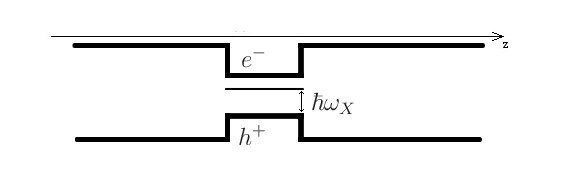
\includegraphics[scale=.5]{QW.jpg}
 \end{figure}
  $$\omega_X(k) = \omega_X^0 + \frac{\hbar k^2}{2m_X}$$
  \end{frame}

 

\begin{frame}{Dinamica}

  Gradi di libertà sul piano $xy$
  \begin{itemize}
  %   \item {
%     Interazioni tra fotoni per effetti non lineari:\\
%     \centerline{
%         $ \chi^{(3)}\quad \rightarrow \quad$ four-wave mixing
%     }
%   }\end{itemize}
  \item { fotoni
   \begin{flalign*}
   \ham_{cav} = \intk \hbar \omega_C (k) \ \oa_C^\dagger \oa_C  &&
  \end{flalign*}
  }
  
    \item { eccitoni, con interaz. di dipolo (RWA)
 \begin{flalign*} 
    \ham_{exc} = \intk \hbar \omega_X (k) \ \oa_X^\dagger  \oa_X ~ + ~\hbar \Omega_R \left(\oa_C^\dagger \oa_X + \oa_X^\dagger \oa_C\right) &&
 \end{flalign*}
   }
  \end{itemize}
  
 
  \begin{equation*}
  \boxed{
   \ham_{free} = \hbar \displaystyle \intk 
      \begin{pmatrix} \oa_C^\dagger & \oa_X^\dagger \end{pmatrix}\,
      \begin{pmatrix} \omega_C & \Omega_R \\ \Omega_R & \omega_X \end{pmatrix}\,\begin{pmatrix}\oa_C \\ \oa_X \end{pmatrix}
      }
  \end{equation*}
 

%   %%%%%%%% 	LA PORCHERIA 	che però funziona
%    \vspace{-.25cm}
%    \hline
%    \vspace{.1cm}
%    {\Large$$\Downarrow$$\par}
%    %$$\Downarrow$$
%    \vspace{-.25cm}
   
  \end{frame}

\begin{frame}{Polaritoni liberi}

\begin{equation*}
%\begin{align}
 \ham_{free} = \hbar \intk \omega_{LP} (k) \oa_{LP}^\dagger \oa_{LP} ~ + ~ \omega_{UP} (k) \oa_{UP}^\dagger \oa_{UP}
%\end{align}
\end{equation*}

\begin{minipage}{\textwidth}
\begin{columns}
\footnotesize{
  \begin{column}{.4\textwidth}
  
   $$\begin{cases}
	\oa_C = C\lp \ \oa\lp + C\up \ \oa\up \\
	\oa_X = X\lp \ \oa\lp + X\up \ \oa\up
     \end{cases}
   $$
   
   Coefficienti di Hopfield

   \begin{equation*}
    \begin{align}
      &\omega_{(UP,LP)} (k) = \frac{\omega_C (k) + \omega_X (k)}{2} \\
			     &\pm \left[\Omega_R^2 + \left(\frac{\omega_C (k) - \omega_X (k)}{2}\right)^2\right]^{1/2}
    \end{align}
   \end{equation*}
   Dispersione
  \end{column}
  }
  \hspace{.5cm}
  \begin{column}{.55\textwidth}
   \begin{figure}[h]
    \includegraphics[scale=.2]{polaritons.png}
   \end{figure}

  \end{column}
\end{columns}
\end{minipage}

 

  
  

\end{frame}



\subsection{Interazioni}

% You can reveal the parts of a slide one at a time
% with the \pause command:
\begin{frame}{Second Slide Title}
  \begin{itemize}
  \item {
    First item.
    \pause % The slide will pause after showing the first item
  }
  \item {   
    Second item.
  }
  % You can also specify when the content should appear
  % by using <n->:
  \item<3-> {
    Third item.
  }
  \item<4-> {
    Fourth item.
  }
  % or you can use the \uncover command to reveal general
  % content (not just \items):
  \item<5-> {
    Fifth item. \uncover<6->{Extra text in the fifth item.}
  }
  \end{itemize}
\end{frame}

\subsection{Pumping \& losses}

\section{Teoria di campo medio}
\subsection{Stato stazionario}

\begin{frame}{Blocks}
\begin{block}{Block Title}
You can also highlight sections of your presentation in a block, with it's own title
\end{block}
\begin{theorem}
There are separate environments for theorems, examples, definitions and proofs.
\end{theorem}
\begin{example}
Here is an example of an example block.
\end{example}
\end{frame}

\subsection{Spettro delle eccitazioni}

\section{Superfluidità}
\subsection{Resonant Raileigh Scattering}
\subsection{Criterio di Landau}
\subsection{Verifica sperimentale}

% Placing a * after \section means it will not show in the
% outline or table of contents.
\section*{Summary}

\begin{frame}{Summary}
  \begin{itemize}
  \item
    The \alert{first main message} of your talk in one or two lines.
  \item
    The \alert{second main message} of your talk in one or two lines.
  \item
    Perhaps a \alert{third message}, but not more than that.
  \end{itemize}
  
  \begin{itemize}
  \item
    Outlook
    \begin{itemize}
    \item
      Something you haven't solved.
    \item
      Something else you haven't solved.
    \end{itemize}
  \end{itemize}
\end{frame}



% All of the following is optional and typically not needed. 
\appendix
\section<presentation>*{\appendixname}
\subsection<presentation>*{For Further Reading}

\begin{frame}[allowframebreaks]
  \frametitle<presentation>{For Further Reading}
    
  \begin{thebibliography}{10}
    
  \beamertemplatebookbibitems
  % Start with overview books.

  \bibitem{Author1990}
    A.~Author.
    \newblock {\em Handbook of Everything}.
    \newblock Some Press, 1990.

    
  \beamertemplatearticlebibitems
  % Followed by interesting articles. Keep the list short. 

  \bibitem{Someone2000}
    S.~Someone.
    \newblock On this and that.
    \newblock {\em Journal of This and That}, 2(1):50--100,
    2000.
  \end{thebibliography}
\end{frame}

\end{document}


